\documentclass[12pt]{article}
\usepackage{polski}
\usepackage[utf8]{inputenc}
\usepackage{amsmath}
\usepackage{mathtools}
\usepackage[thinc]{esdiff}
\usepackage{graphicx}
\usepackage{hyperref}
\usepackage[yyyymmdd]{datetime}
\newtheorem{theorem}{Twierdzenie}
\renewcommand{\dateseparator}{-}
\hypersetup{
	colorlinks=true,
	linkcolor=blue,
	filecolor=magenta,      
	urlcolor=cyan,
}

\addtolength{\textwidth}{3cm}
\addtolength{\hoffset}{-1.5cm}
\addtolength{\textheight}{3cm}
\addtolength{\voffset}{-1.5cm}

\begin{document}
	\begin{center}
		\Huge
		\textbf{Crazy Eights}
		
		\LARGE
		Instrukcja do gry
	\end{center}

	\section*{Autorzy i podział pracy}
	
	Jakub Gałązka - 25\%
	
	\noindent Odpowiedzialny za: logika gry, struktura projektu, algorytm botów, szeroko pojęty backend
	
	\noindent\rule{\textwidth}{0.4pt}
	
	\noindent Grzegorz Stefański - 25\%
	
	\noindent Odpowiedzialny za: testy, zarządzanie repozytorium, raportowanie, szeroko pojęty backend
	
	\noindent\rule{\textwidth}{0.4pt}
	
	\noindent Krzysztof Pysz - 25\%
	
	\noindent Odpowiedzialny za: layout graficzny, interfejs GUI
	
	\noindent\rule{\textwidth}{0.4pt}
	
	\noindent Andrzej Opaliński - 25\%
	
	\noindent Odpowiedzialny za: oprawa graficzna, interfejs GUI
	
	\section*{Instrukcja}
	
	\begin{figure}[h]
		\centering
		\renewcommand*{\figurename}{Fig.} 
		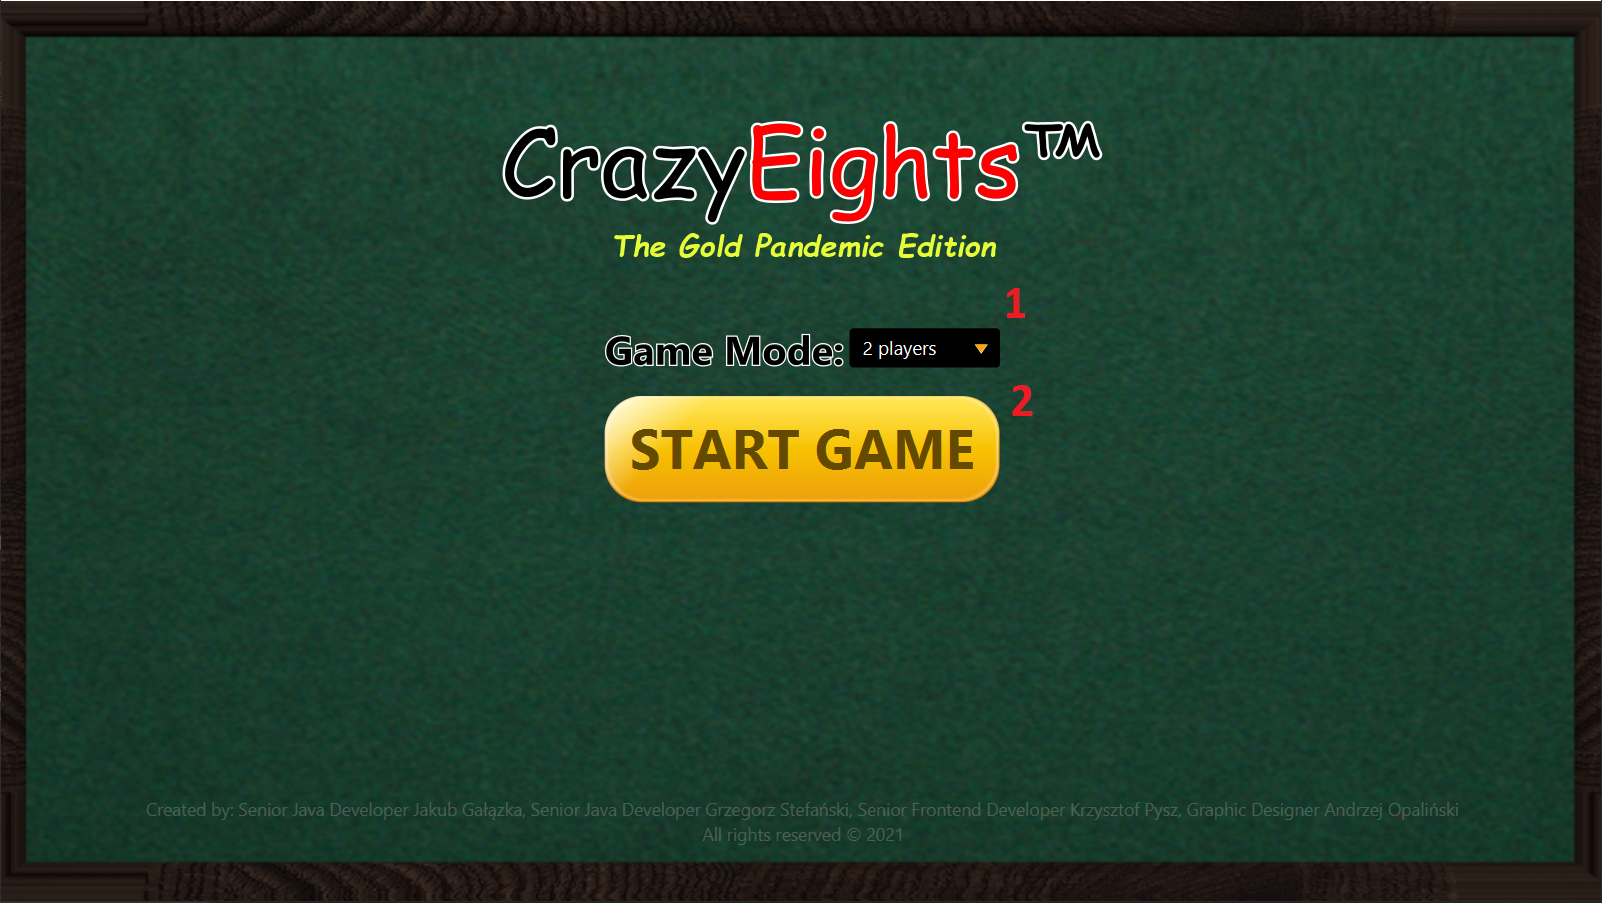
\includegraphics[width=\textwidth]{img/menu.png}
		\caption{Screen z menu gry.}
		\label{}
	\end{figure}
	
	\begin{enumerate}
		\item Wybór rodzaju gry. Możliwa jest gra na 2, 3 i 4 graczy. Nie licząc gracza to odpowiednie opcje odpowiadają 1, 2 lub 3 botom będącym naszymi przeciwnikami.
		\item Przycisk rozpoczęcia gry.
	\end{enumerate}

	\begin{figure}[h]
		\centering
		\renewcommand*{\figurename}{Fig.} 
		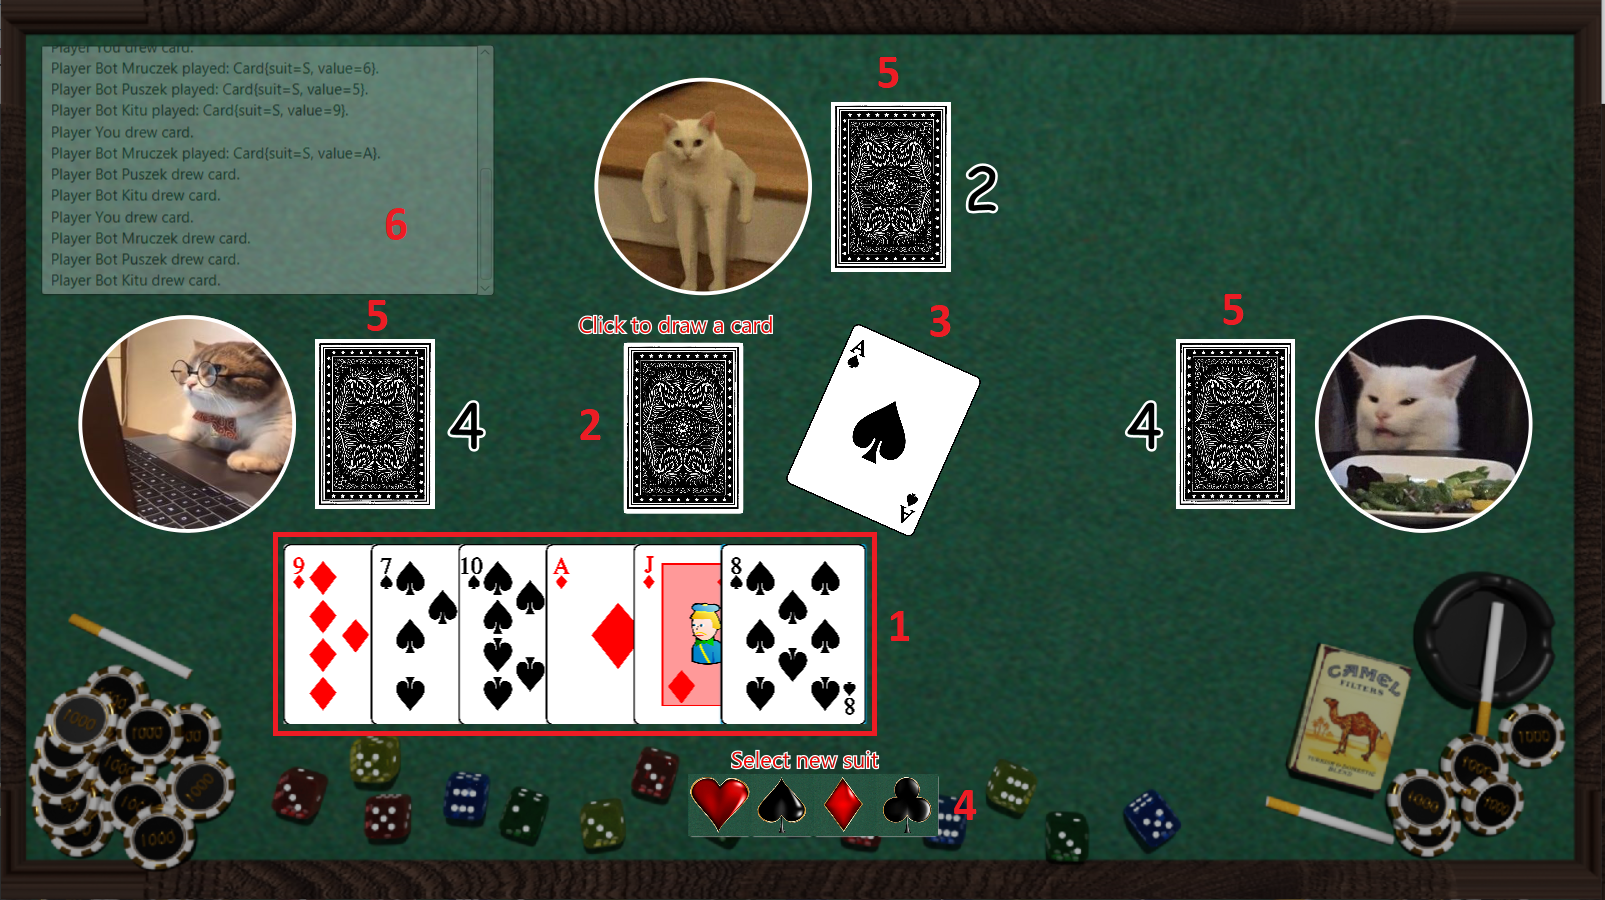
\includegraphics[width=\textwidth]{img/game.png}
		\caption{Widok w grze po rozpoczęciu gry dla 4 graczy.}
		\label{}
	\end{figure}

	\begin{enumerate}
		\item Karty które gracz ma na ręce. Kliknięcie na jedną z kart powoduje jej zagranie o ile pozwalają na to zasady gry.
		\item Talia kart po której naciśnięciu dobieramy karty.
		\item Stos kart odrzuconych. Zawsze na nim jest widoczna ostatnia odrzucona karat przez gracza lub botów. Do tej karty należy zagrywać karty z ręki.
		\item Okno wyboru nowego koloru po zagraniu szalonej ósemki. Domyślnie niewidocznie. Pojawia się po kliknięciu na szaloną ósemkę.
		\item Stosy kart botów z licznikiem pozostałych ich kart na ręce.
		\item Okno zdarzeń zawierające informacje o wszystkich wykonanych ruchach.
	\end{enumerate}

	\paragraph{GitGub repository: \href{https://github.com/GrzegorzStefanski-ib/CrazyEights.git}{click to go}} 
	
\end{document}